\subsection{Pengujian Sistem \textit{Flexible Control}}

Pada bagian ini akan dijelaskan tentang tujuan, skenario, hasil, dan analisis dari pengujian sistem sekaligus komponen \textbf{\textit{Flexible Control}}.

\subsubsection{Tujuan Pengujian}

Tujuan pengujian ini memastikan sistem \textbf{\textit{Flexible Control}} dapat berjalan dengan baik dan menghasilkan perilaku yang sesuai.

\subsubsection{Skenario Pengujian}

Pengujian terhadap komponen \textbf{\textit{Flexible Control}} dilakukan dengan beberapa skenario sebagai berikut serta ekspektasi dari pengujian yang dilakukan.
\begin{enumerate}
    \item \bfseries Sebuah \textit{rule} memenuhi kondisi untuk mengubah alokasi prosesor.\normalfont
    
    Prosesor akan berubah jumlahnya sesuai dengan \textit{rule} yang memenuhi kondisi. Perubahan pada spesifikasi \textit{pods} juga diekspektasikan mengikuti.

    \item \bfseries Sebuah \textit{rule} memenuhi kondisi untuk mengubah alokasi memori.\normalfont
    
    Prosesor akan berubah jumlahnya sesuai dengan \textit{rule} yang memenuhi kondisi. Perubahan pada spesifikasi \textit{pods} juga diekspektasikan mengikuti. Memory Used Percent akan menurun karena penambahan yang terjadi.
\end{enumerate}

\subsubsection{Hasil Pengujian dan Analisis}

Pengujian akan dilakukan dengan \textit{file rule} yang dapat dilihat pada gambar \ref{fig:ac-rule}. Terdapat dua buah \textit{rule} yang akan diuraikan sebagai berikut.

\begin{enumerate}
    \item Jika \textit{load average 1m} pada 10 detik kedepan diprediksikan diatas 0 maka akan ditambah alokasi prosesor sebesar 1000m atau sejumlah 1. Kondisi dari \textit{rule} sengaja dibuat seperti itu agar rule pasti terpenuhi.
    \item Jika \textit{memory used percent} pada 5 dan 10 detik kedepan diprediksikan diatas 60 maka akan ditambah alokasi memori sebesar 2048 mebibyte atau sejumlah 2 gibibyte (Gi). Kondisi dari \textit{rule} sengaja dibuat seperti itu agar rule pasti terpenuhi.
\end{enumerate}

Hasil dari pengujian skenario kedua dapat dilihat pada gambar \ref{fig:ac-mem}. Dan perubahan terhadap spesifikasi pods dapat dilihat pada gambar \ref{fig:ac-mem-kube}. Perubahan juga terjadi pada \textit{memory used percent} pada \textit{stream file} atau data yang ditarik oleh komponen \textbf{\textit{Metrics Fetcher}} dapat dilihat pada gambar \ref{fig:ac-mf-turun}.
Diikuti dengan hasil dari pengujian skenario pertama dapat dilihat pada gambar \ref{fig:ac-cpu}. Dapat dilihat bahwa prosesor berubah sesuai dengan ekspektasi. Perubahan pada spesifikasi \textit{pods} juga mengikuti perubahan prosesor yang dapat dilihat pada gambar \ref{fig:ac-cpu-kube}.

\begin{figure}[h]
    \centering
    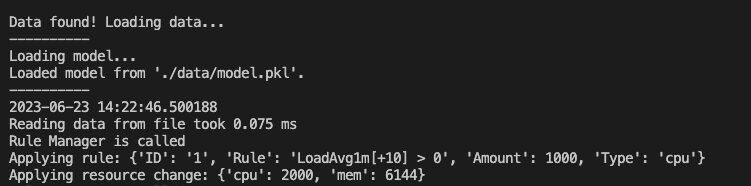
\includegraphics[width=0.8\textwidth]{chapter-4/ac-cpu.png}
    \caption{Hasil Pengujian Komponen \textit{Flexible Control} Skenario 1: Perubahan Prosesor}
    \label{fig:ac-cpu}
\end{figure}

\begin{figure}[h]
    \centering
    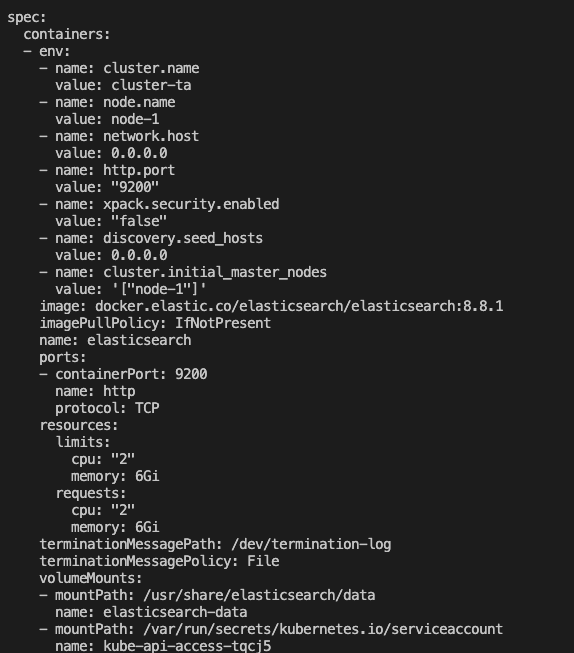
\includegraphics[width=0.8\textwidth]{chapter-4/ac-cpu-kube.png}
    \caption{Hasil Pengujian Komponen \textit{Flexible Control} Skenario 1: Perubahan Spesifikasi Kubernetes}
    \label{fig:ac-cpu-kube}
\end{figure}

\begin{figure}[h]
    \centering
    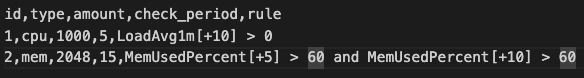
\includegraphics[width=0.8\textwidth]{chapter-4/ac-rule.png}
    \caption{File Rule untuk Pengujian Komponen \textit{Flexible Control}}
    \label{fig:ac-rule}
\end{figure}

\begin{figure}[h]
    \centering
    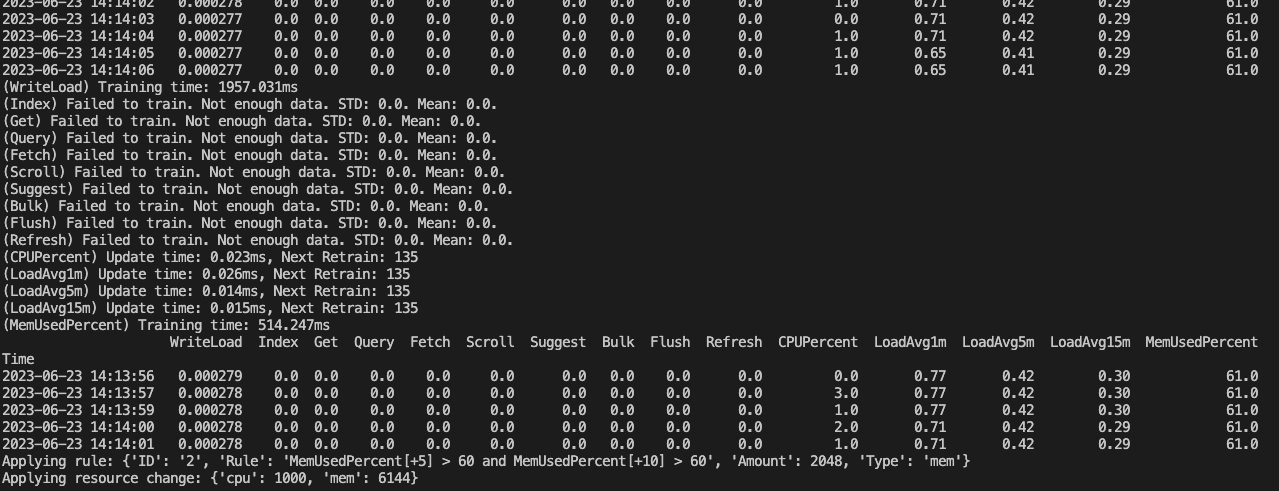
\includegraphics[width=0.8\textwidth]{chapter-4/ac-mem.png}
    \caption{Hasil Pengujian Komponen \textit{Flexible Control} Skenario 2: Perubahan Memori}
    \label{fig:ac-mem}
\end{figure}

\begin{figure}[h]
    \centering
    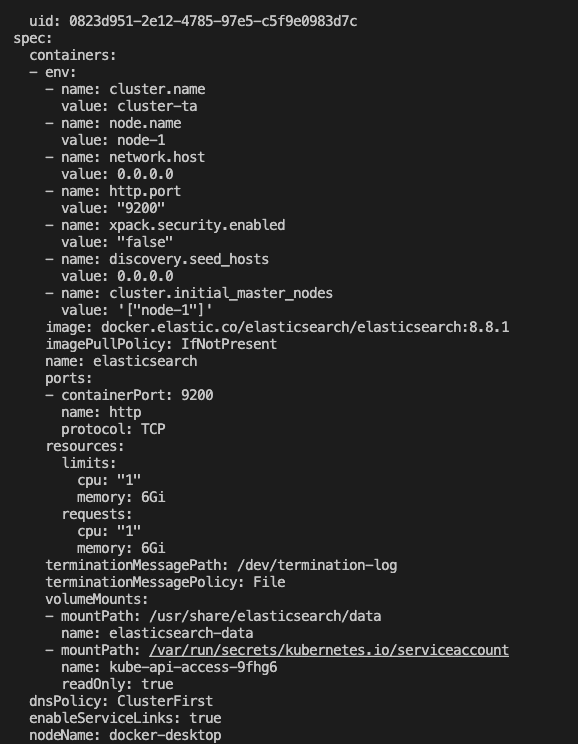
\includegraphics[width=0.8\textwidth]{chapter-4/ac-mem-kube.png}
    \caption{Hasil Pengujian Komponen \textit{Flexible Control} Skenario 2: Perubahan Spesifikasi Kubernetes}
    \label{fig:ac-mem-kube}
\end{figure}

\begin{figure}[h]
    \centering
    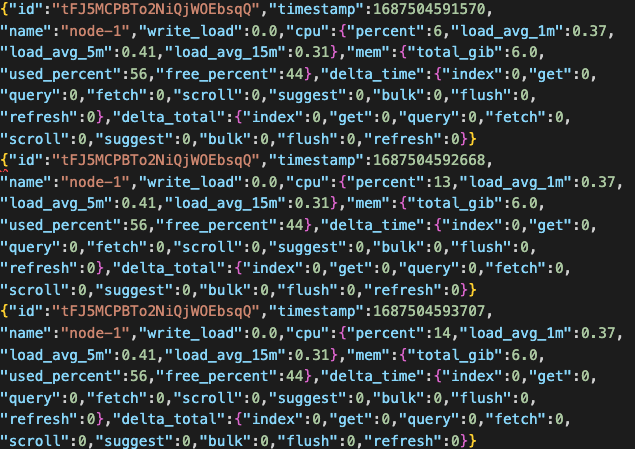
\includegraphics[width=0.8\textwidth]{chapter-4/ac-mf-turun.png}
    \caption{Hasil Pengujian Komponen \textit{Flexible Control} Skenario 2: Perubahan Memory Used Percent pada \textit{stream file}}
    \label{fig:ac-mf-turun}
\end{figure}

Maka untuk pengujian komponen \textbf{\textit{Flexible Control}} sudah sesuai ekspektasi dan sistem dapat berjalan dengan baik.